\chapter{外部トリガを用いた応答評価試験}
この章では,外部トリガを用いた粒子線に対する応答評価試験について述べる.\ref{sec:extsetup}節で外部トリガでデータ取得をする際のセットアップ,\ref{sec:exthow}節で手順,\ref{sec:extconc}節で取得データ結果を示し,\ref{sec:selfsum}節で考察を行なっている.

\section{外部トリガを用いた応答評価試験概要}
この節では,4chip-RD53Aモジュールに対して行われる品質試験について述べる.\ref{sec:masspro}節で述べたように,現在現在実機で用いるモジュールを量産するための準備として,プロトタイプ版のASICが4 $\mathrm{Chip}$搭載された4chip-RD53Aモジュールで量産体制の確認が計画されている.この時に,バンプボンディングに異常が無いかを確認するための試験が,外部トリガを用いた応答評価試験である.現在計画されている試験は,クーリングボックスと呼ばれる,温度が低温に維持された小さな箱の中で行い,トリガには前章で述べたHitOR信号ではなく,シンチレータからの光信号を用いる.計画されている外部トリガを用いた応答評価試験セットアップを図\ref{fig:trigplan}に示す.

\begin{figure}[h]
  \centering
  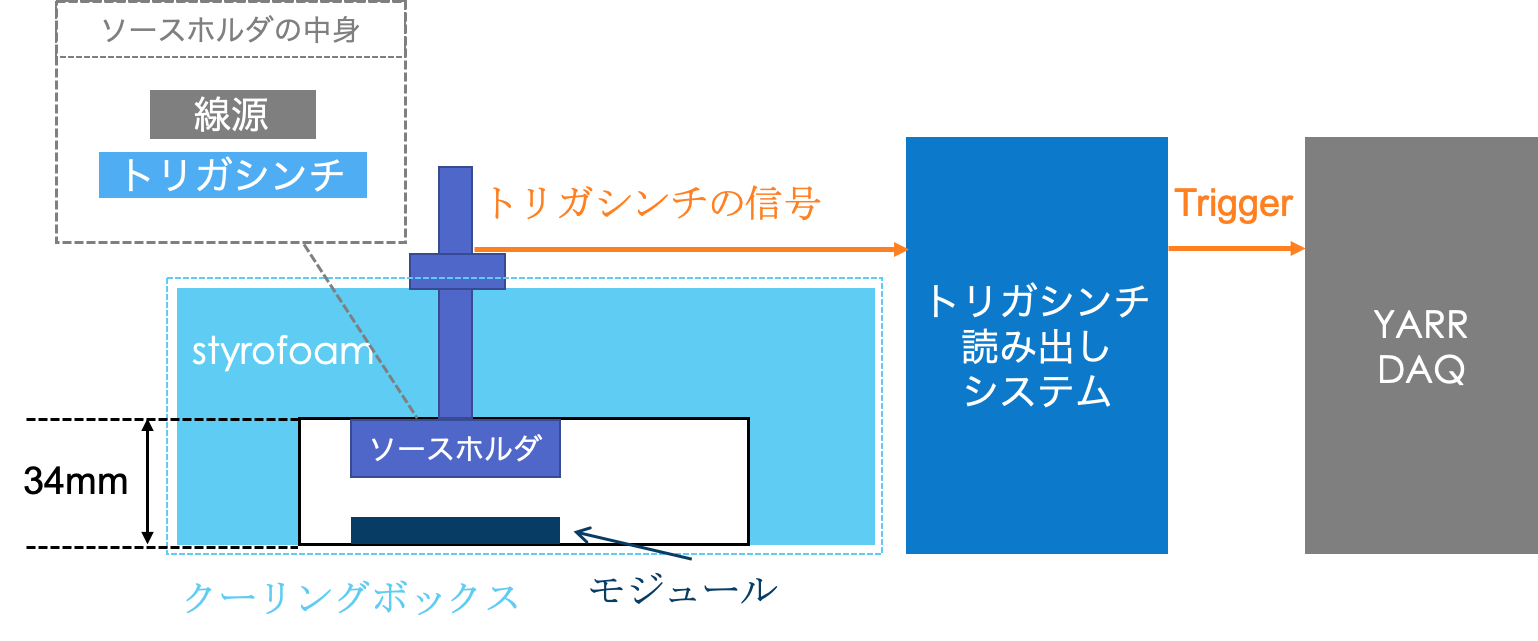
\includegraphics[width=12cm]{./figure/trigplan.png}
  \caption{計画されている外部トリガを用いた応答評価試験セットアップ}
  \label{fig:trigplan}
\end{figure}

線源とモジュールの間にシンチレータを配置し,そのシンチレータに粒子が入射した時の発光をMPPCで検出し信号として読み出すことで,トリガに用いる.このシンチレータとMPPCが合わさったものを以降トリガシンチと呼ぶ.トリガシンチは非常にコンパクトな環境で用いられることや,線源とモジュールの間に配置されることから,なるべく小さく,粒子線を遮ることのないように薄くあることが要求されている.

\section{トリガシンチの基礎測定}
この節では,RD53Aに対して行われる品質試験で外部トリガとして使用されるトリガシンチの性能の基礎測定について述べる.

\subsection{概要}
今回使用したシンチレータと,光を読み出すためにMPPCをシンチレータに取り付けた様子を図\ref{fig:trigscin}に示す.図中のライトガイドとは,シンチレータに粒子が入射した時に発光した光を効率よくMPPCまで伝えるための部品である.また,\ref{sec:trigplan}でも述べたように,非常にコンパクトな環境での利用を目的としているため,トリガシンチは箱の中,読み出し回路は箱の外で使用される.そのため,MPPCの足は約30 $\mathrm{cm}$のケーブルをはんだづけすることで延長し,MPPCからの信号を箱の外まで伝えられるようにしてある.シンチレータは0.5 $\mathrm{mm}$と非常に薄いものを使用し,MPPCと共に黒テープで遮光を行なった.

\begin{figure}[h]
  \centering
  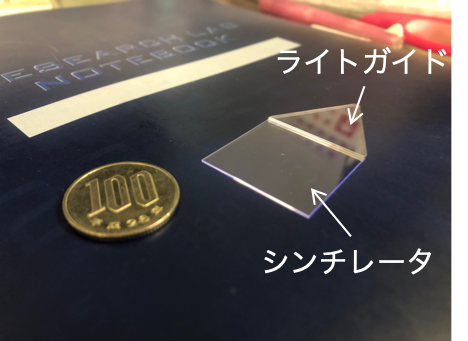
\includegraphics[width=6cm]{./figure/trigscin.png}
  \caption{0.5mmのシンチレータの様子}
  \label{fig:trigscin}
\end{figure}


このトリガシンチに対して以下の2点に関する基礎測定を行なった.
\begin{itemize}
\item トリガレート 
\item MPPCが読み出した光量と粒子線が入射した位置の依存性
\end{itemize}

また,今回は使用が予定されている環境がコンパクトな環境なため,ライトガイドを用いた場合と用いなかった場合で,トリガレートや光量に差がないのであれば,ライトガイドはない方が望ましい.よって,ライトガイドが無い場合についても同様の点について基礎測定を行なった.

\subsection{基礎測定のセットアップ}
図\ref{fig:trigsetup}に読み出しシステムの概要を示す.主に,シンチレータとMPPC,読み出し基板,ADCモジュールで構成している.シンチレータで発光した光をMPPCで検出し,読み出し回路でデジタル信号として読み出す.読み出し基板とADCモジュールはコネクタを通してLEMOケーブルで接続している.

\begin{figure}[h]
  \centering
  \includegraphics[width=8cm]{./figure/trigsetup.png}
  \caption{トリガシンチの基礎測定セットアップ}
  \label{fig:trigsetup}
\end{figure}

\subsubsection*{MPPCからの信号を波形整形する基板}
本研究を行うにあたって,MPPCからの信号を波形整形する基板を作成した.基板を図\ref{fig:extcircle}に示す.主に,電圧供給回路,反転増幅回路,コンパレータ回路,LVDS変換回路から構成されている.基板はKiCADというCERN開発のオープンソースプリント基板CADを用いて設計・作成した.LEMO1からは増幅されたMPPCのアナログ信号を,LEMO2からはコンパレータによって閾値電圧と比較することで変換されたデジタル信号を,DPからはTTLだったデジタル信号が変換されてLVDS出力のデジタル信号を読み出すことができる.その3点についてオシロスコープで観測した波形を図\ref{fig:extosiro}に示す.


\subsection{トリガレートの測定}
トリガシンチの上に線源を配置した時としない時で,トリガレートの比較を行なった.


\subsection{光量と粒子の入射位置の依存性測定}
トリガシンチの上に

\section{外部トリガを用いた応答評価試験セットアップ}
\label{sec:extsetup}
RD53Aの量産にあたって,行われる品質試験では,外部トリガを用いた応答評価試験が行われる.そのため,実際に行われる試験環境に近いセットアップで試験を行なった.セットアップの写真を以下に示す.MPPCには58$\mathrm{V}$印加した.SCCとFPGAボード,PCを用いてシステムを組む大枠は変わらずに,線源の配置とトリガに使用するものが異なっている.\par
実際に行われる試験は,クーリングボックスと呼ばれる,温度が低温に維持された小さな箱の中で行い,トリガには前章で述べたHitOR信号ではなく,シンチレータからの光信号を用いる.シンチレータは線源とモジュールの間に設置するため,なるべく$\beta$線を遮らないように,厚みは0.5$\mathrm{mm}$と非常に薄いものを使用した.
実際に行われる試験環境はクーリングボックスと呼ばれる,温度が低温に維持された小さな箱の中で行う.それに合う応答評価試験セットアップを考えるにあたって,線源とシンチレータ,シンチレータの光信号を電気信号に変換するMPPCが乗ったソースホルダと,MPPCからのアナログ信号を波形整形し,LVDSのデジタル信号に変換するような基板の設計を行なった.

\subsection{ソースホルダの設計}
ソースホルダの外観を以下に示す.クーリングボックス内で使用することを想定し,コンパクトな作りになっている.これは,FreeCADというオープンソース汎用3D CADモデラで設計し,3Dプリンタを用いて作成した.

\subsection{MPPCからの信号を波形整形する回路}

\subsubsection*{回路の動作確認}
MPPCからの信号を正しく波形整形できているかをオシロスコープを用いて確認した.増幅されたMPPCからの信号がコンパレータによって,デジタル信号に変換され,TTL to LVDS変換のチップによって,差動信号に変換されている様子がわかる.

\section{トリガシンチの基礎測定}
この回路では,信号を出力をコンパレータの閾値によって設定している.この閾値によって,MPPCからの信号が削られることなく伝達されているかを確認した.

\section{応答評価試験手順}
\label{sec:exthow}
\section{応答評価試験結果}
\label{sec:extconc}
\section{考察}
\label{sec:extsum}
